%************VERSUCHSDURCHFÜHRUNG & MESSERGEBNISSE***********
\section{Execution}
\label{sec:execution}

This sections serves as documentation on how the results as described in Section \ref{sec:summary} might be reproduced. Instructions are based on the assumption that an environment with suitable equipment such as described in Sections \ref{sec:setup} and \ref{sec:equipment} is used and set up accordingly.

\subsection{Laser Source and Safety}

All experimental steps described in subsequent sections require the infrared laser source to be operational, for which the main switch needs to be activated. Additionally, there is a cover at the output of the laser source blocking the outgoing beam that needs to be opened during measurement.

For safety reasons, this cover is to remain closed while changes to the setup are made. Furthermore, safety goggles need to be used and reflective apparel such as watches or rings need to be removed. The eyes of the experimentators must strictly remain well above the path of the laser beams.

\subsection{Beam Positioning}

For the laser beam to be measured by the grating spectrometer, it needs to be directed from the output of the laser source towards the input aperture of the spectrometer. This is achieved by directing it via a series of dielectric mirrors, which are positioned and aligned such that on one hand the SHG stage and the iodine cell can be traversed by the beam, while on the other hand the beam reaches the aperture of the spectrometer in a correct angle.

As described in Section \ref{sec:setup}, the bases for the optical elements used in this experiment can be positioned and fixed on a grid of tapped holes. While the bases allow for vertical adjustment as well as crude rotation with respect to the vertical axis, the mounts allow for fine-tuned vertical and horizontal tilting of the mirrors, thus enabling alignment of the laser beam as desired.

One strategy that proves to be advantageous is to locate the mirrors in such a way that the beam follows a path containing only angles of approximately \SI{90}{\degree}, for which the reflection angle relative to each mirror is approximately \SI{45}{\degree}. For this approach the grid of tapped holes in the table can be used as a rough reference, while additionally the sensitivity for changes in mirror angle are minimized.

As shown in Figure \ref{fig:execution:aperture}, the grating spectrometer exhibits a dedicated adjustable mirror for directing the laser beam towards the aperture. There are covers at both the mirror and the aperture, each containing a special hole to be used for properly adjusting the laser beam while the covers are closed. When correctly adjusted, the laser beam hits both the hole at the mirror as well as the hole at the cover of the aperture. During measurement, the cover at the mirror is always to be opened.

\begin{figure}[H]
    \centering
    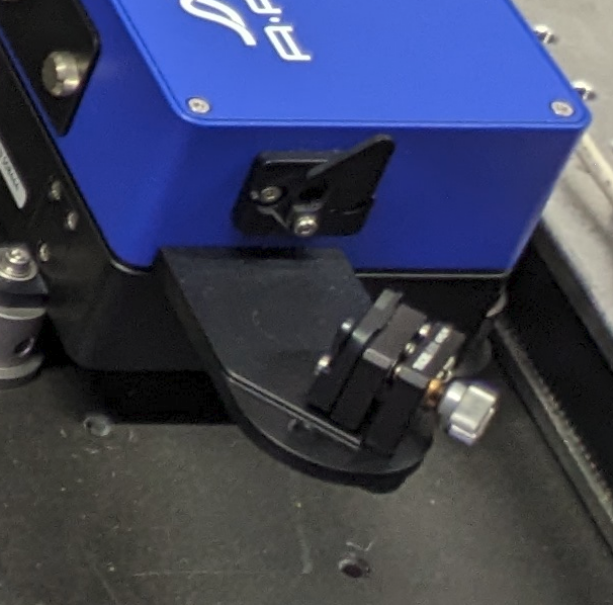
\includegraphics[width=0.45\textwidth]{graphics/aperture.png}
    \caption{Aperture and dedicated mirror at the grating spectrometer.}
    \label{fig:execution:aperture}
\end{figure}


The overall procedure for directing the beam towards the spectrometer as desired involves stepwise adjustment of the mirrors starting from the laser source and going towards the spectrometer, followed by iterative fine-tuning of each mirror both in height and rotation.

\subsection{Measurement Procedure}



% \label{sec:versuchsandordnung}

% \begin{table}[H]
%     \centering
%     \caption{Messung Zählimpulse bei bestimmten Zeitpunkten (ein Ausschnitt davon) mit Na-22-Quelle. \\
%     $i$ = Messindex, $t$ = Zeitpunkt, $z$ = Zählimpulse}
%     \label{tab:execution:durch:zaehlstatistik}
%     \begin{tabular}{cccccc}
%     \hline
%     $i$ / 1 & $t$ / s & $z$ / cps \\ \hline
%     1 & 1  & 440  \\
%     2 & 2 & 389 \\
%     3 & 3 & 433 \\
%     4 & 4,1 & 395 \\
%     5 & 5 & 392 \\
%     \vdots & \vdots & \vdots  \\
%     313 & 313  & 413  \\
%     314 & 314 & 377 \\
%     315 & 315 & 432 \\
%     316 & 316 & 416 \\
%     317 & 317,1 & 415 \\ \hline
%     \end{tabular}
%     \end{table}

% \begin{figure}[H]
%     \centering
%     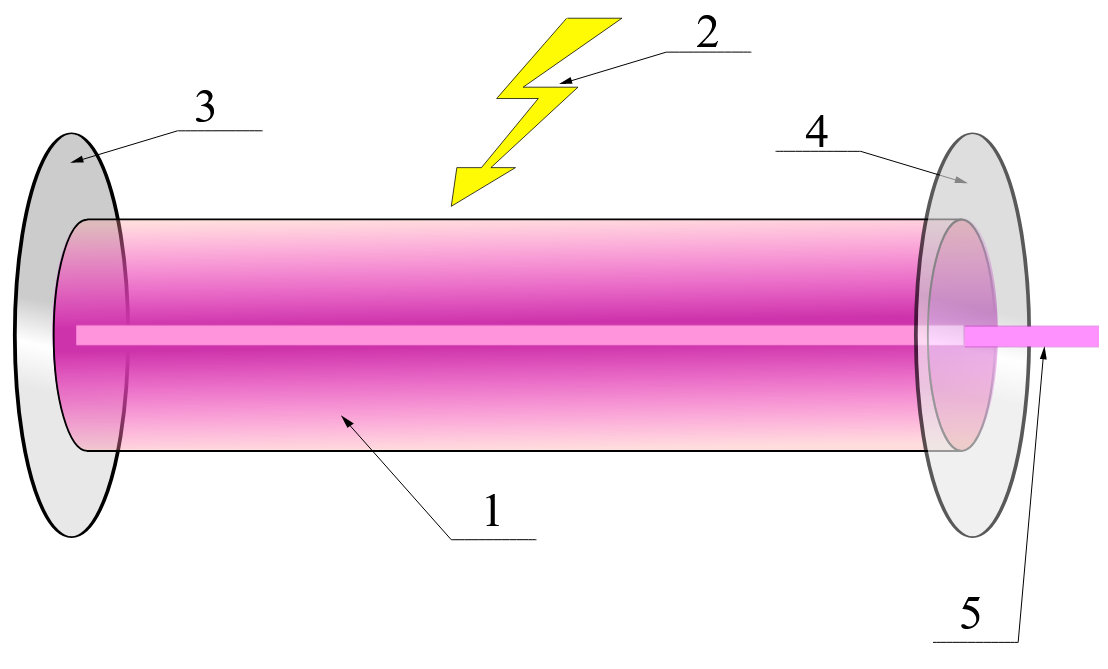
\includegraphics[width=\textwidth]{graphics/Laser_Cavity.png}
%     \caption{Aufnahme der Zählstatistik mit Digitalzähler. \\
%     vertikal = Zerfälle pro Sekunde, horizontal = Messindex}
%     \label{fig:execution:durchfuehrung:zaehlstatistik}
% \end{figure}